Die optischen Besonderheiten von glänzenden Oberflächen faszinieren zahlreiche Menschen.
So wird Glanz bereits seit Jahrhunderten mit Luxus und Reichtum verbunden.
Dieser Zusammenhang wird durch den imposanten Spiegelsaal im Schloss von Versailles untermauert (siehe Abbildung \ref{img:spiegelSaal}).
Nach langer Bauzeit im 17. Jahrhundert bildete dieser Saal die Hauptattraktion des Schlosses und zieht heute noch sehr viele Touristen an \cite{versailles}.

% Abbildung: Spiegelsaal
{
	\begin{figure}[H]
		\centering
		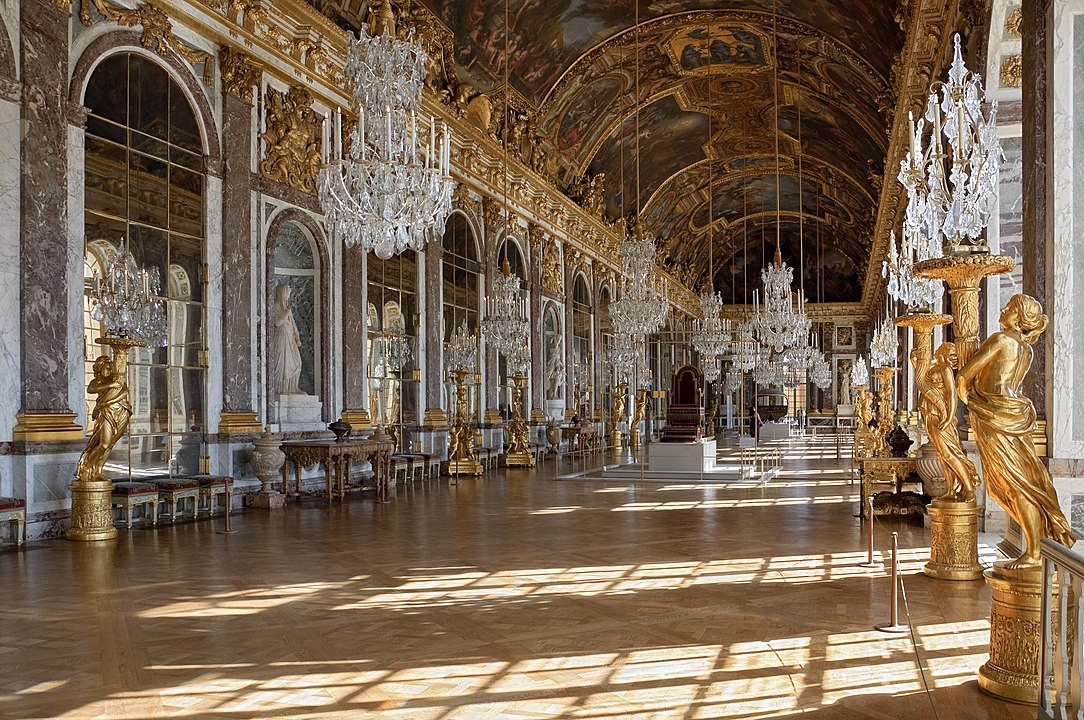
\includegraphics[width=0.5\textwidth]{01_einfuehrung/figures/spiegelSaal}
		\caption[Spiegelsaal im Schloss von Versailles]{Spiegelsaal im Schloss von Versailles}
		\label{img:spiegelSaal}
	\end{figure}
}

\noindent
Bereits Neugeborene fühlen sich den Reflexionen von Glanzobjekten hingezogen \cite{shinyObjects}.
Verhaltensforscher stellten anhand von Studien die Theorie auf, dass die Zuneigung zu spiegelnden Objekten evolutionär bedingt ist.
Durch die Reflexionen auf den Oberflächen soll man glänzende Objekte mit Wasser assoziieren \cite{waterAndShininess}.
Auch die industriellen Bereiche wollen diese Faszination der Leute ansprechen.
So befinden sich an vielen Stellen im Alltag glänzende Oberflächen, um Menschen zu begeistern.
Z. B. in der Automobilindustrie werden täglich große Karosserieflächen glänzend lackiert.
Alleine in Deutschland wurden in den Jahren von 1990 bis 2021 im Durchschnitt ungefähr 5 Millionen Personenkraftwagen pro Jahr produziert \cite{statistaPKW}.
Ein großer Teil der Fahrzeuge erhält nach der Lackierung eine spiegelnde Oberfläche.
Solche Oberflächen müssen zur Qualitätssicherung durch besondere Verfahren auf Defekte überprüft werden.
Dabei stellen sich diese anziehenden Spiegelungen als Probleme heraus.
Die spekularen Reflexionen sorgen dafür, dass nicht direkt die spiegelnden Oberflächen, sondern die verzerrten Spiegelbilder der Umgebungen betrachtet werden.
Somit schaut man z. B. in Abbildung \ref{img:spiegelndeKarosserie} auf die Karosserieoberfläche, doch sieht darin das verzerrte Spiegelbild des Streifenmusters oder des Roboterarms.

% Abbildung: Beschriftung Delle
{
	\begin{figure}[H]
		\centering
		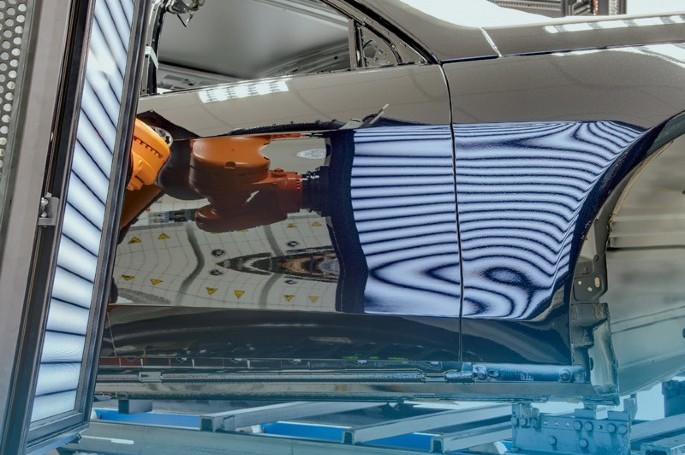
\includegraphics[width=0.5\textwidth]{01_einfuehrung/figures/spiegelndeKarosserie}
		\caption[Spiegelnde Karosserieoberfläche]{Spiegelung der Umgebung auf der Karosserieoberfläche \cite{spiegelndeKarosserieImg}}
		\label{img:spiegelndeKarosserie}
	\end{figure}
}

\noindent
Die riesige Menge an produzierten Bauteilen und die hohen Qualitätsanforderungen machen eine automatisierte Prüfung der Teile unumgänglich.
Dabei stoßen die üblichen Verfahren der industriellen Bildverarbeitung auf ihre Grenzen, sodass neue Methoden eingeführt werden müssen.
Diese speziellen Anwendungen erfordern den Einsatz von deflektometrischen Prüfaufbauten, die sich die Spiegelung von bestimmten Szenen zunutze machen.
In der Industrie sind solche Verfahren schon seit Längerem zur Analyse der Topografie von spiegelnden Freiformflächen etabliert.
Deflektometrische Verfahren funktionieren nach einem ähnlichen Prinzip wie auch die Inspektion von spiegelnden Oberflächen durch Prüfpersonal. 
Durch die Reflexionen und Verzerrungen auf glänzenden Oberflächen schließt man auf die Form und Krümmung der Oberfläche.
Das wissenschaftliche Gebiet der Deflektometrie ist auch heute noch Thema für viele Forschungsarbeiten und wird stetig weiterentwickelt.

%Problemstellung und Zielsetzung
{
	\FloatBarrier
    \section{Problemstellung und Zielsetzung}
    \label{sec:problemstellung}
    Im Rahmen der Arbeit werden spekular reflektierende Objektoberflächen unter Abbildung von bekannten Mustern durch eine Kamera aufgenommen, anschließend ausgewertet und auf Defekte überprüft.
Welche Informationen können aus der Beobachtung von Spiegelbildern gewonnen werden?
Wie sehen allgemein anwendbare Methoden aus, um spiegelnde Oberflächen qualitativ zu bewerten?
Das Ziel der Arbeit ist es, diese Fragen zu erforschen und aufzuklären.
Des Weiteren sollen ein Aufbau, die Ansteuerung von Beleuchtung und Kamera und die notwendige Auswertung des Bildmaterials entwickelt werden, durch welche eine Erkennung von Oberflächendefekten ermöglicht wird.
Die Umsetzung soll dabei in Form einer Softwareerweiterung, eines sogenannten \textit{Plug-ins}, für NeuroCheck erfolgen.

\p
Während der Arbeit soll außerdem auch ein bestimmter Sonderfall betrachtet werden - transparente Prüfobjekte.
Die Problematik ist dabei, dass man neben der Reflexion des Lichts mit der Transmission zu kämpfen hat.
Wie auch bei den regulären deflektometrischen Verfahren ist das Ziel, anhand einer verzerrten Szene Aussagen über die Oberflächenbeschaffenheit zu treffen.
Für die transparenten Objekte gibt es dafür verschiedene Lösungsansätze, um den negativen Einflüssen der Transmission entgegenzuwirken.
}

%Aufbau der Bachelorarbeit
{
	\FloatBarrier
    \section{Aufbau der Bachelorarbeit}
    \label{sec:aufbauDerArbeit}
    Die Arbeit wird zur Bearbeitung der Frage- und Problemstellungen in sechs Kapitel unterteilt.

\p
Im zweiten Kapitel soll sich mit den theoretischen Grundlagen zur Entwicklung von deflektometrischen Verfahren befasst werden.

\p
Im Anschluss werden in Kapitel \ref{chp:sichtpruefungDurchLichtstreuung} und \ref{chp:deflektometrischeRegistrierung} zwei deflektometrische Verfahren beschrieben, um die Fragestellungen der Thesis bearbeiten zu können.
\p
Das fünfte Kapitel dient der Erfassung und Diskussion der Ergebnisse, die durch die eingeführten Verfahren und verwendeten Aufbauten erreicht werden können.

\p
Das letzte Kapitel soll einen Überblick der erzielten Erkenntnisse dieser Arbeit schaffen und einen Ausblick auf zukünftige Verbesserungen der vorgestellten Verfahren geben.
}

%Unternehmensvorstellung
{
	\FloatBarrier
    \section{Unternehmensvorstellung}
    \label{sec:unternehmensvorstellung}
    Die vorliegende Bachelorarbeit wird in Kooperation mit der Hochschule für Technik Stuttgart bei der NeuroCheck GmbH angefertigt.

\p
Die NeuroCheck GmbH ist ein Unternehmen, welches System- und Softwarelösungen im Fachgebiet der industriellen Bildverarbeitung anbietet.
Dabei blickt das Unternehmen mit Hauptsitz in Remseck am Neckar auf eine Firmengeschichte von über 25 Jahren zurück.
Mit nun mehr als 20000 verkauften Applikationen in über 40 Ländern sowie mehreren Partnerunternehmen im Ausland haben die NeuroCheck-Systeme weltweit Anwendungen gefunden.

\p
Mithilfe der NeuroCheck-Software ist es möglich, automatisierte Sichtprüfungen zur Qualitätskontrolle durchzuführen.
Hierfür lassen sich vom Anwender komplexe Prüfprogramme nach einem Baukastenprinzip erstellen.
Dadurch entstehen vielseitige An\-wen\-dungs\-mög\-lich\-kei\-ten.
Diese schaffen weite Teile der Industriebranchen als mögliche Kunden, unter anderem die Automobilindustrie, die Elektronikbranchen und die Medizintechnik.

% Abbildung: NeuroCheck Logo
\begin{figure}[H]
	\centering
	
\includegraphics[width=0.3\textwidth]{01_einfuehrung/unternehmensvorstellung/figures/neurocheck_logo}
	\caption[NeuroCheck Logo]{NeuroCheck Logo \cite{nclogo}}
\end{figure}
}